\section{Hamiltonian\&The LS-coupling scheme without fine structure}

\begin{frame}{Hamiltonian}
\uncover<1->{
    \begin{block}{The central-field approximation}
        \begin{equation*}
            \begin{aligned}
                V_{\mathrm{CF}}\left(r\right)&=-\frac{Ze^2/4\pi\epsilon_0}r+S(r),\\
                H_{\mathrm{CF}}&=\sum_{i=1}^N\left\{-\frac{\hbar^2}{2m}\nabla_i^2+V_{\mathrm{CF}}\left(r_i\right)\right\}.
            \end{aligned}
        \end{equation*}
    \end{block}}
\uncover<2->{
    The residual electrostatic interaction:
    \begin{equation*}
        H_{\mathrm{re}}=\sum_{i=1}^N\left\{\sum_{j>i}^N\frac{e^2/4\pi\epsilon_0}{r_{ij}}-S(r_i)\right\},
    \end{equation*}}
\uncover<3->{
    Hamiltonian:
    \begin{equation*}
        H=H_{\mathrm{CF}}+H_{\mathrm{re}}+H_{\mathrm{s-o}}.
    \end{equation*}}
\end{frame}

\begin{frame}{Hamiltonian}
\uncover<1->{
    It is generally very difficult to calculate the eigenvalues of the above Hamiltonian, so two extremes are usually discussed.}
    \begin{enumerate}
        \item<2-> LS-coupling scheme:
        \begin{equation*}
            H_{\mathrm{s-o}}\ll H_{\mathrm{re}}: H_{\mathrm{s-o}}{\to}\text{perturbation}, \text{basic quantum numbers}: LSJM_J,
        \end{equation*}
        \item<3-> jj-coupling scheme:
        \begin{equation*}
            H_{\mathrm{s-o}}\gg H_{\mathrm{re}}: H_{\mathrm{re}}{\to}\text{perturbation}, \text{basic quantum numbers}: n_il_ij_iJM_J.
        \end{equation*}
    \end{enumerate}
\end{frame}

\begin{frame}{LS-coupling scheme without fine structure}
\uncover<1->{
    \begin{block}{Hamiltonian}
        \begin{equation*}
            \begin{aligned}
                H&=\sum_{i=1}^N\left[-\frac{\hbar^2}{2m}\nabla_i^2+V_{\mathrm{CF}}\left(r_i\right)+\left\{\sum_{j>i}^N\frac{e^2/4\pi\epsilon_0}{r_{ij}}-S(r_i)\right\}\right],\\
                H&=H_{\mathrm{CF}}+H_{\mathrm{re}}.
            \end{aligned}
        \end{equation*}
    \end{block}}
\uncover<2->{
    Consider
    \begin{equation*}
        \boldsymbol{L}=\sum_i\boldsymbol{l}_i,\quad\boldsymbol{S}=\sum_i\boldsymbol{s}_i,\quad\boldsymbol{J}=\boldsymbol{L}+\boldsymbol{S}.
    \end{equation*}}
\uncover<3->{
    No external torque:
    \begin{equation*}
        \left[\boldsymbol{L}^2,H_\mathrm{re}\right]=0\quad\mathrm{~and~}\quad\left[{L}_z,H_\mathrm{re}\right]=0\mathrm.
    \end{equation*}}
\uncover<4->{
    $H_\mathrm{re}$ doesn't depend on spin:
    \begin{equation*}
        \left[\boldsymbol{S}^2,H_\mathrm{re}\right]=0\quad\mathrm{~and~}\quad\left[{S}_z,H_\mathrm{re}\right]=0.
    \end{equation*}}
\end{frame}

\begin{frame}{LS-coupling scheme without fine structure}
\uncover<1->{
    Therefore,
    \begin{equation*}
        \begin{aligned}
            \text{good quantum numbers}&: L,M_L,S,M_S,\\
            \text{eigenstates of} H_\mathrm{re}&: \ket{LM_LSM_S}.
        \end{aligned}
    \end{equation*}}
\uncover<2->{
    Label: 
    \begin{equation*}
        \textbf{terms}: {}^{2S+1}L_J.
    \end{equation*}}
\uncover<3->{
    \begin{block}{e.g. 3p4p in silicon}
        \begin{equation*}
            \begin{aligned}
                l_{1}&=1,& l_{2}&=1&\Rightarrow\quad L&=0,1\mathrm{~or~}2,\\
                s_{1}&=\frac{1}{2},& s_{2}&=\frac{1}{2}&\Rightarrow\quad S&=0\mathrm{~or~}1,\\
            \end{aligned}
        \end{equation*}
        \begin{equation*}
            \text{terms (without J) }:\quad {}^{2S+1}L={}^{1}\mathrm{S,}^{1}\mathrm{P,}^{1}\mathrm{D,}^{3}\mathrm{S,}^{3}\mathrm{P,}^{3}\mathrm{D}.
        \end{equation*}
    \end{block}}
\end{frame}

\begin{frame}{Energy levels}
\uncover<1->{
    Isotropy: degeneracy with respect to $M_L$ and $M_S$.}
    \begin{columns}
    \hspace*{1em}
    \column{0.51\textwidth}<2->
        \begin{figure}
            \centering
            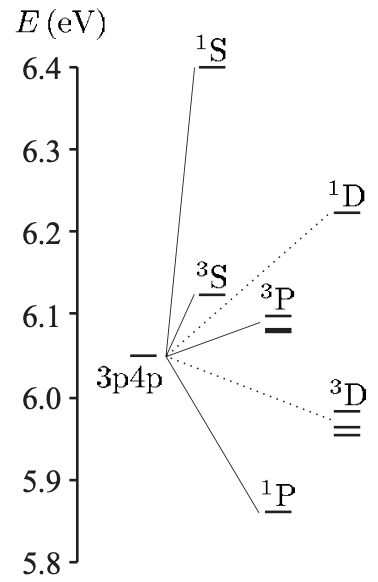
\includegraphics[scale=0.32]{fig/fig 5.1.png}
            \caption{3p4p in silicon}
        \end{figure}
        \begin{block}{Degenerate states}
            \begin{equation*}
                (2l_1+1)(2l_2+1)(2s_1+1)(2s_2+1)=36.
            \end{equation*}
        \end{block}
    \column{0.5\textwidth}<3->
        \begin{figure}
            \centering
            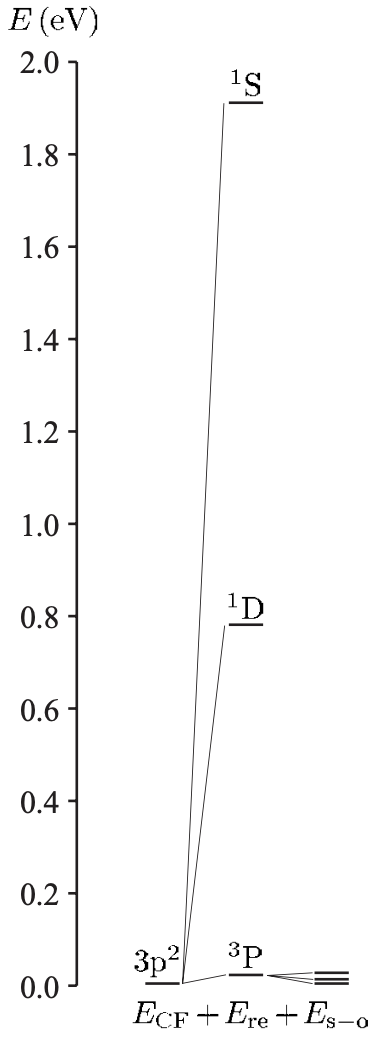
\includegraphics[scale=0.32]{fig/fig 5.2.png}
            \caption{$\mathrm{3p}^2$ in silicon}
        \end{figure}
    \end{columns}
\end{frame}